\documentclass{homeworg}
\usepackage{enumitem}
\usepackage{listings}
\usepackage{color} %red, green, blue, yellow, cyan, magenta, black, white
\definecolor{mygreen}{RGB}{28,172,0} % color values Red, Green, Blue
\definecolor{mylilas}{RGB}{170,55,241}
\usepackage{xcolor,cancel}

\newcommand\hcancel[2][black]{\setbox0=\hbox{$#2$}%
\rlap{\raisebox{.45\ht0}{\textcolor{#1}{\rule{\wd0}{1pt}}}}#2}

%\usepackage{authblk}
%\title{CSE 5301 - HW02}
%\author[1]{Bardia Mojra}
%\affil[1]{1000766739}
\begin{document}

% --------------- Title -------------------------------------
%\maketitle
\begin{center}
\textbf{EE 5323 - HW03}\\
\end{center}

\noindent
Bardia Mojra\\
1000766739\\
\today\\
HW03 -- Nonlinear System Simulations\\
EE 5323 -- Nonlinear Systems\\
Dr. Lewis

\exercise
\noindent
\textbf{Voltera Predator-Prey System} \\
Consider the Voltera predator-prey system,\\
\begin{equation*}
\dot{x}_1 = - x_1 + x_1 x_2
\end{equation*}
\begin{equation*}
\dot{x}_2 = x_2 -  x_1 x_2
\end{equation*}
Find the equilibrium points and their nature.\\

\noindent
\textbf{Answer} \\
State variable is given as:
\begin{equation*}
~\dot{x}_1 = - x_1 + x_1 x_2
\end{equation*}
\begin{equation*}
~\dot{x}_2 = x_2 -  x_1 x_2
\end{equation*}

The Voltera predator-prey system has limit cycles therefore the system is
at equilibrium when the population of both predator and prey remain
constant; thus, the derivative should be zero.
To find the equilibrium, I set $\dot{x}_{1}=0$ and $\dot{x}_{2}=0$.
Solve the system for its roots.\\

\begin{equation*}
~\dot{x}_1 = 0 \Rightarrow 0 =  - x_1 + x_1 x_2
\end{equation*}
\begin{equation*}
~\dot{x}_2 = 0 \Rightarrow 0 = x_2 -  x_1 x_2
\end{equation*}
\begin{equation*}
~0 = x_1 (\beta x_2 - \alpha)~\Rightarrow~x_1 = 0 ; ~x_2 = \alpha/\beta
\end{equation*}
\begin{equation*}
  ~0 = x_2 (\gamma - \sigma x_1)~\Rightarrow~x_1 = \gamma/\sigma ; ~x_2 = 0
\end{equation*}

There are two equilibrium points at $(x_1,~x_2)$,

\begin{itemize}
  \item At zero, $~(0 ,~ 0),$
  \item Any positive pair of integers $(\alpha/\beta,~\gamma/\sigma)$
\end{itemize}

The equilibrium point nature of the zero is a stable center point that is a
limit cycle. The other e.p. has a saddle point nature because it is stable
in one dimension (goes to zero) and unstable in the other (goes to
infinity).

\lstset{language=Matlab,%
    %basicstyle=\color{red},
    breaklines=true,%
    morekeywords={matlab2tikz},
    keywordstyle=\color{blue},%
    morekeywords=[2]{1}, keywordstyle=[2]{\color{black}},
    identifierstyle=\color{black},%
    stringstyle=\color{mylilas},
    commentstyle=\color{mygreen},%
    showstringspaces=false,%without this there will be a symbol in the places where there is a space
    numbers=left,%
    numberstyle={\tiny \color{black}},% size of the numbers
    numbersep=9pt, % this defines how far the numbers are from the text
    emph=[1]{for,end,break},emphstyle=[1]\color{red}, %some words to emphasise
    %emph=[2]{word1,word2}, emphstyle=[2]{style},
}
\newpage
\noindent
\textbf{Matlab Code}\\
\lstinputlisting{hw03_Q01_code.m}
\newpage
\noindent
\textbf{Figures}\\
\begin{figure}[h]
  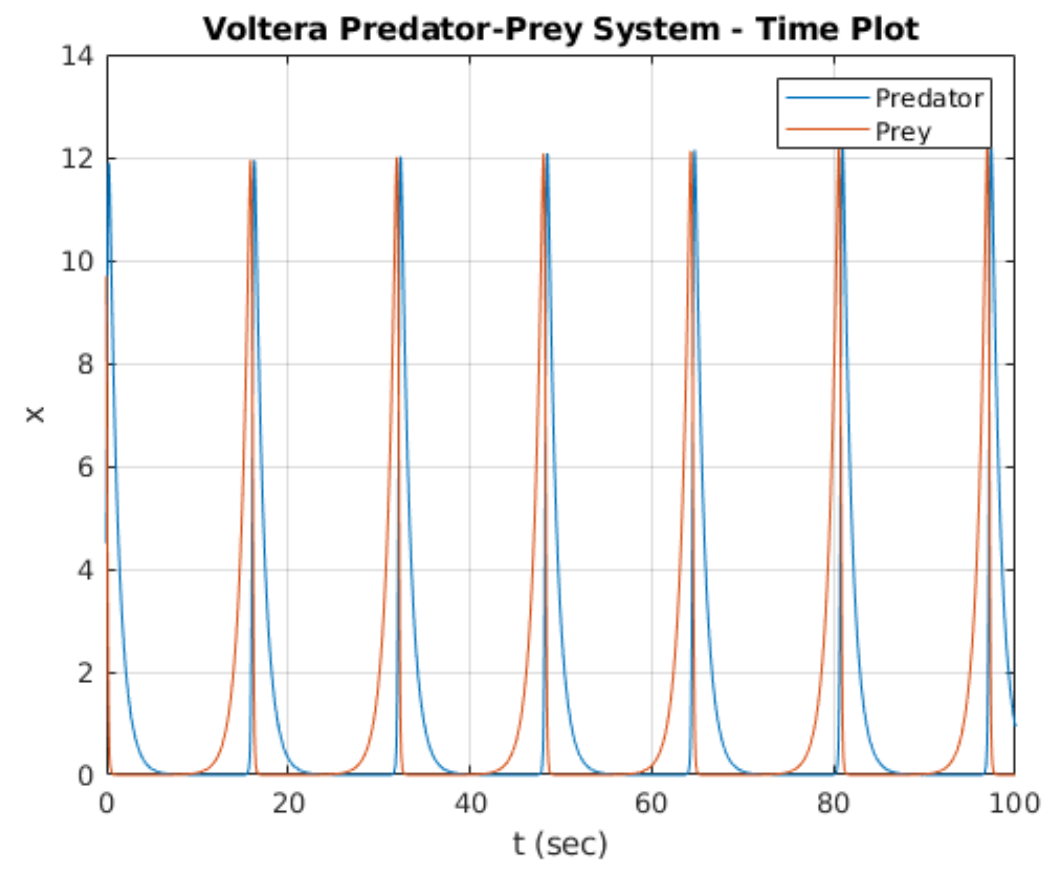
\includegraphics[width=.6\textwidth]{fig001.png}
  \centering
\end{figure}
\begin{figure}[h]
  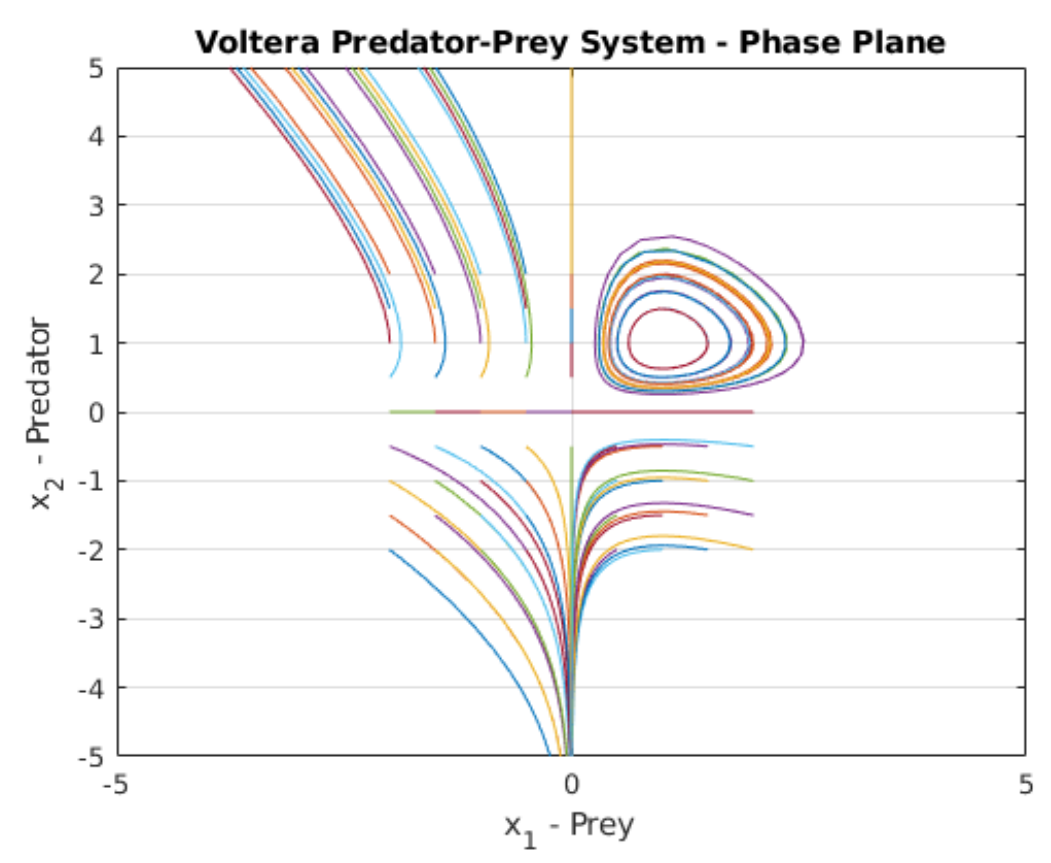
\includegraphics[width=.6\textwidth]{fig002.png}
  \centering
\end{figure}

\exercise
\noindent
\textbf{Equilibrium points and linearization} \\
Consider the following system,\\
\begin{equation*}
\dot{x}_1 = x_2 (-x_1 + x_2 -1)
\end{equation*}
\begin{equation*}
\dot{x}_2 = x_1 (x_1 + x_2 + 1)
\end{equation*}

\begin{enumerate}[label=(\alph*)]
\item Find all equilibrium points
\item Find Jacobian
\item Find the nature of all e.p.s
\end{enumerate}

\noindent
\textbf{Answer} \\
\noindent
a. Find all e.p.s\\
At equilibrium points, all states reach their minimal energy state; therefore,
the derivative of the state should equal zero. Then, we solve for the roots of
the obtained characteristic equation.

\begin{equation*}
f(x_1,~x_2) = \dot{X} = 0 \Rightarrow~~
  \begin{cases}
    \dot{x}_1 = 0 \Rightarrow~~ x_2(-x_1 + x_2 -1)=0\\
    \dot{x}_2 = 0 \Rightarrow~~ x_1(~~x_1 + x_2 + 1)=0\\
  \end{cases}
\end{equation*}
\noindent
There are four possible cases for state derivative, $\dot{X}$, to equal zero,
$\dot{X}=0$; where the system is at an equilibrium point.\\ \\
\noindent
\textbf{Case 1}
\begin{equation*}
    \begin{cases}
      (x_2=0)\hcancel{(-  x_1 + x_2 -1)}=0\\
      (x_1=0)\hcancel{(~~x_1 + x_2 + 1)}=0\\
    \end{cases}
\end{equation*}
\noindent
e.p. at $(x_1 , x_2) = (0,0)$\\

\noindent
\textbf{Case 2}
\begin{equation*}
    \begin{cases}
      (x_2=0)\hcancel{(-  x_1 + x_2 -1)}=0\\
      \hcancel{(x_1)}(~~x_1 + x_2 + 1 =0)=0 \Rightarrow x_1 = -1
    \end{cases}
\end{equation*}
\noindent
e.p. at $(x_1 , x_2) = (-1,0)$\\

\noindent
\textbf{Case 3}
\begin{equation*}
    \begin{cases}
      \hcancel{(x_2)}(-  x_1 + x_2 -1=0)=0 \Rightarrow x_2 = +1\\
      (x_1=0)\hcancel{(~~x_1 + x_2 + 1 =0)}=0
    \end{cases}
\end{equation*}
\noindent
e.p. at $(x_1 , x_2) = (0,+1)$\\

\noindent
\textbf{Case 4}
\begin{equation*}
    \begin{cases}
      \hcancel{(x_2)}(-  x_1 + x_2 -1 =0)=0 \\
      \hcancel{(x_1)}(~~~x_1 + x_2 + 1 =0)=0 \\
    \end{cases}
\end{equation*}
\begin{equation*}
\Rightarrow x_2 = 0 ; \Rightarrow x_1 = -1 \text{ \ as in \textbf{Case 2} or \textbf{Case 3}}
\end{equation*}

\noindent
b. Find the Jacobian\\


\begin{equation*} %\label{eq:2}
  f(x_1,~x_2) =
  \begin{cases}
    x_2 (-x_1 + x_2 -1)\\
    x_1 (~~~x_1 + x_2 + 1)\\
  \end{cases}
  = \dot{X} = AX
\end{equation*}


\begin{equation*} %\label{eq:2}
\dot{X} =
  \begin{bmatrix}
    \frac{d f}{d x_1} & \frac{d f}{d x_2}
  \end{bmatrix}
  \begin{bmatrix}
    x_1 \\
    x_2 \\
  \end{bmatrix}
  \Rightarrow
  \dot{X} =
  \begin{bmatrix}
    \frac{d }{d x_1}(-x_2) & \frac{d }{d x_2}(x_2 - 1) \\
    \frac{d }{d x_1}(x_1 +1) & \frac{d }{d x_2}(x_1)
  \end{bmatrix}
  \begin{bmatrix}
    x_1 \\
    x_2 \\
  \end{bmatrix}
  \Rightarrow
\end{equation*}

\begin{equation*}
  \dot{X}  = AX \Rightarrow
  \dot{X} =
  \begin{bmatrix}
    -x_2 & 0 \\
    0 & x1 \\
  \end{bmatrix}
  \begin{bmatrix}
    x_1 \\
    x_2 \\
  \end{bmatrix}
  \Rightarrow
\end{equation*}

\begin{equation*}
  A =
  \begin{bmatrix}
    -x_2 & 0 \\
    0 & x1 \\
  \end{bmatrix}
\end{equation*}


\noindent
c. Find the nature of all e.p.s,\\
Compute the poles of the system using Eigen values,

\begin{equation*}
\bigtriangleup (s) = | SI - A| =
\begin{vmatrix}
  s+x_2 & 0 \\
  0 & s-x_1 \\
\end{vmatrix}
\Rightarrow
\end{equation*}
\begin{equation*}
(s+x_2)(s-x_1)=0 \Rightarrow
\begin{cases}
  s=~x_1\\
  s=~-x_2\\
\end{cases}
\end{equation*}
\begin{equation*}
  (s+x_2)(s-x_1)=0 \Rightarrow s^2 - x_1 x_2 s - x_1 x_2 = 0
\end{equation*}

\noindent
Standard form for characteristic equation,
\begin{equation*}
  s^2 + 2 \alpha s + \alpha^2 + \beta^2 = s^2 + 2 \alpha s + \omega_n^2 = 0 \\
  ; ~~\beta = j \omega
\end{equation*}

\noindent
Case 1, at $(0,0)$; $s^2 = 0~\Rightarrow~s=0$, center point with poles at the origin on the s-plane.\\
\noindent
Case 2, at $(-1,0)$; $s=1$ and $s=0$, center point with poles at the origin and +1 on the s-plane.\\
\noindent
Case 3, at $(0,+1)$; $s=0$ and $s=-1$, center point with poles at -1 and the origin on the s-plane.\\


\exercise
\noindent
\textbf{System simulation} \\
Consider the following system,\\
\begin{equation*}
\dot{x}_1 = x_2 (-x_1 + x_2 -1)
\end{equation*}
\begin{equation*}
\dot{x}_2 = x_1 (x_1 + x_2 + 1)
\end{equation*}

\noindent
Simulate the system using MATLAB for various initial conditions for the two cases:
\begin{enumerate}[label=(\alph*)]
  \item Take ICs spaced in a uniform mesh in the box x1=[-10,10], x2=[-10,10]. Make one phase
  plane plot with all the trajectories on it. Plot phase plane on square [-15,15]x[-15,15].
  \item Take ICs spaced in a uniform mesh in the box x1=[-3,3], x2=[-3,3]. Make one phase
  plane plot with all the trajectories on it. Plot phase plane on square [-5,5]x[-5,5].
\end{enumerate}

\noindent
\textbf{Answer} \\
\noindent
a. The phase plane rotation for all test cases are counter-clockwise. \\ \\
\textbf{Matlab Code}
\lstinputlisting{hw03_Q03a_sol.m}
\newpage
\noindent
\textbf{Figures}\\
\begin{figure}[h]
  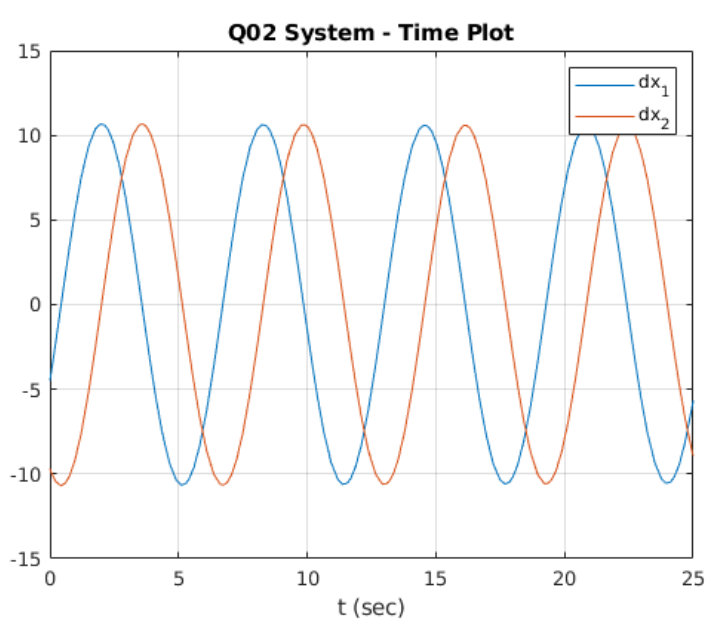
\includegraphics[width=.6\textwidth]{fig003.png}
  \centering
\end{figure}
\begin{figure}[h]
  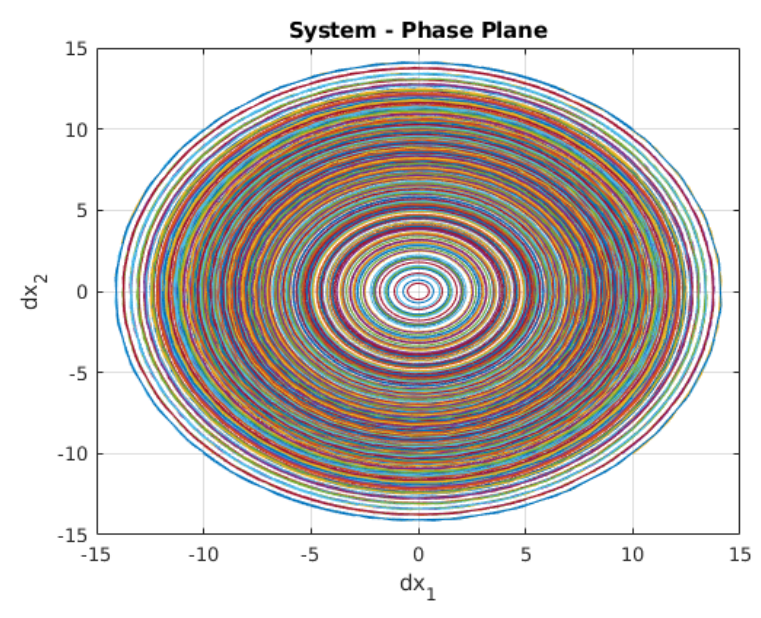
\includegraphics[width=.6\textwidth]{fig004.png}
  \centering
\end{figure}

\newpage
b. The phase plane rotation for all test cases are counter-clockwise.\\ \\
\textbf{Matlab Code}
\lstinputlisting{hw03_Q03b_sol.m}
\newpage
\noindent
\textbf{Figures}\\
\begin{figure}[h]
  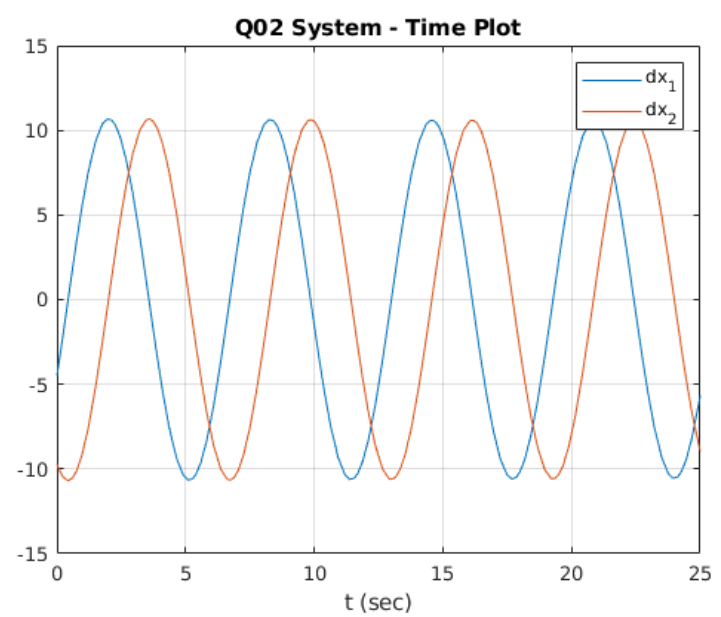
\includegraphics[width=.6\textwidth]{fig005.png}
  \centering
\end{figure}
\begin{figure}[h]
  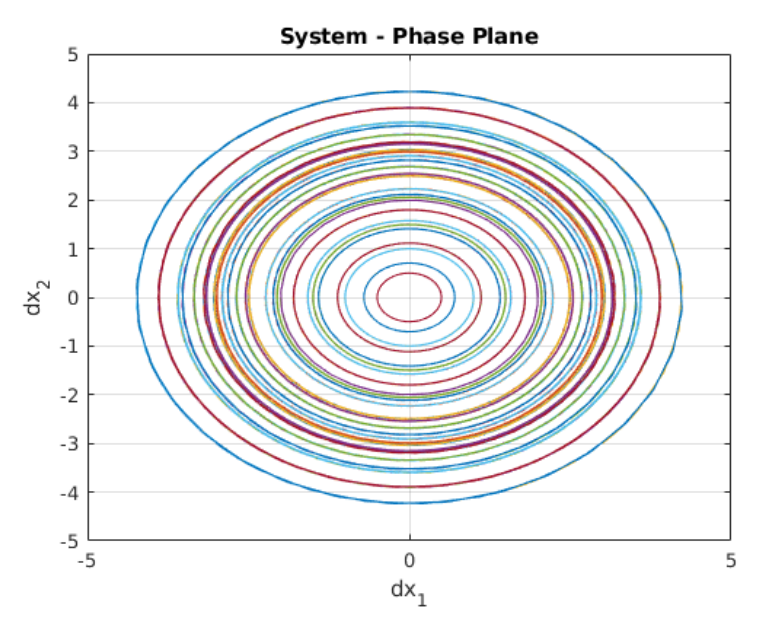
\includegraphics[width=.6\textwidth]{fig006.png}
  \centering
\end{figure}

%\bibliography{ref}

\end{document}
